\documentclass[1p]{elsarticle_modified}
%\bibliographystyle{elsarticle-num}

%\usepackage[colorlinks]{hyperref}
%\usepackage{abbrmath_seonhwa} %\Abb, \Ascr, \Acal ,\Abf, \Afrak
\usepackage{amsfonts}
\usepackage{amssymb}
\usepackage{amsmath}
\usepackage{amsthm}
\usepackage{scalefnt}
\usepackage{amsbsy}
\usepackage{kotex}
\usepackage{caption}
\usepackage{subfig}
\usepackage{color}
\usepackage{graphicx}
\usepackage{xcolor} %% white, black, red, green, blue, cyan, magenta, yellow
\usepackage{float}
\usepackage{setspace}
\usepackage{hyperref}

\usepackage{tikz}
\usetikzlibrary{arrows}

\usepackage{multirow}
\usepackage{array} % fixed length table
\usepackage{hhline}

%%%%%%%%%%%%%%%%%%%%%
\makeatletter
\renewcommand*\env@matrix[1][\arraystretch]{%
	\edef\arraystretch{#1}%
	\hskip -\arraycolsep
	\let\@ifnextchar\new@ifnextchar
	\array{*\c@MaxMatrixCols c}}
\makeatother %https://tex.stackexchange.com/questions/14071/how-can-i-increase-the-line-spacing-in-a-matrix
%%%%%%%%%%%%%%%

\usepackage[normalem]{ulem}

\newcommand{\msout}[1]{\ifmmode\text{\sout{\ensuremath{#1}}}\else\sout{#1}\fi}
%SOURCE: \msout is \stkout macro in https://tex.stackexchange.com/questions/20609/strikeout-in-math-mode

\newcommand{\cancel}[1]{
	\ifmmode
	{\color{red}\msout{#1}}
	\else
	{\color{red}\sout{#1}}
	\fi
}

\newcommand{\add}[1]{
	{\color{blue}\uwave{#1}}
}

\newcommand{\replace}[2]{
	\ifmmode
	{\color{red}\msout{#1}}{\color{blue}\uwave{#2}}
	\else
	{\color{red}\sout{#1}}{\color{blue}\uwave{#2}}
	\fi
}

\newcommand{\Sol}{\mathcal{S}} %segment
\newcommand{\D}{D} %diagram
\newcommand{\A}{\mathcal{A}} %arc


%%%%%%%%%%%%%%%%%%%%%%%%%%%%%5 test

\def\sl{\operatorname{\textup{SL}}(2,\Cbb)}
\def\psl{\operatorname{\textup{PSL}}(2,\Cbb)}
\def\quan{\mkern 1mu \triangleright \mkern 1mu}

\theoremstyle{definition}
\newtheorem{thm}{Theorem}[section]
\newtheorem{prop}[thm]{Proposition}
\newtheorem{lem}[thm]{Lemma}
\newtheorem{ques}[thm]{Question}
\newtheorem{cor}[thm]{Corollary}
\newtheorem{defn}[thm]{Definition}
\newtheorem{exam}[thm]{Example}
\newtheorem{rmk}[thm]{Remark}
\newtheorem{alg}[thm]{Algorithm}

\newcommand{\I}{\sqrt{-1}}
\begin{document}

%\begin{frontmatter}
%
%\title{Boundary parabolic representations of knots up to 8 crossings}
%
%%% Group authors per affiliation:
%\author{Yunhi Cho} 
%\address{Department of Mathematics, University of Seoul, Seoul, Korea}
%\ead{yhcho@uos.ac.kr}
%
%
%\author{Seonhwa Kim} %\fnref{s_kim}}
%\address{Center for Geometry and Physics, Institute for Basic Science, Pohang, 37673, Korea}
%\ead{ryeona17@ibs.re.kr}
%
%\author{Hyuk Kim}
%\address{Department of Mathematical Sciences, Seoul National University, Seoul 08826, Korea}
%\ead{hyukkim@snu.ac.kr}
%
%\author{Seokbeom Yoon}
%\address{Department of Mathematical Sciences, Seoul National University, Seoul, 08826,  Korea}
%\ead{sbyoon15@snu.ac.kr}
%
%\begin{abstract}
%We find all boundary parabolic representation of knots up to 8 crossings.
%
%\end{abstract}
%\begin{keyword}
%    \MSC[2010] 57M25 
%\end{keyword}
%
%\end{frontmatter}

%\linenumbers
%\tableofcontents
%
\newcommand\colored[1]{\textcolor{white}{\rule[-0.35ex]{0.8em}{1.4ex}}\kern-0.8em\color{red} #1}%
%\newcommand\colored[1]{\textcolor{white}{ #1}\kern-2.17ex	\textcolor{white}{ #1}\kern-1.81ex	\textcolor{white}{ #1}\kern-2.15ex\color{red}#1	}

{\Large $\underline{12a_{0263}~(K12a_{0263})}$}

\setlength{\tabcolsep}{10pt}
\renewcommand{\arraystretch}{1.6}
\vspace{1cm}\begin{tabular}{m{100pt}>{\centering\arraybackslash}m{274pt}}
\multirow{5}{120pt}{
	\centering
	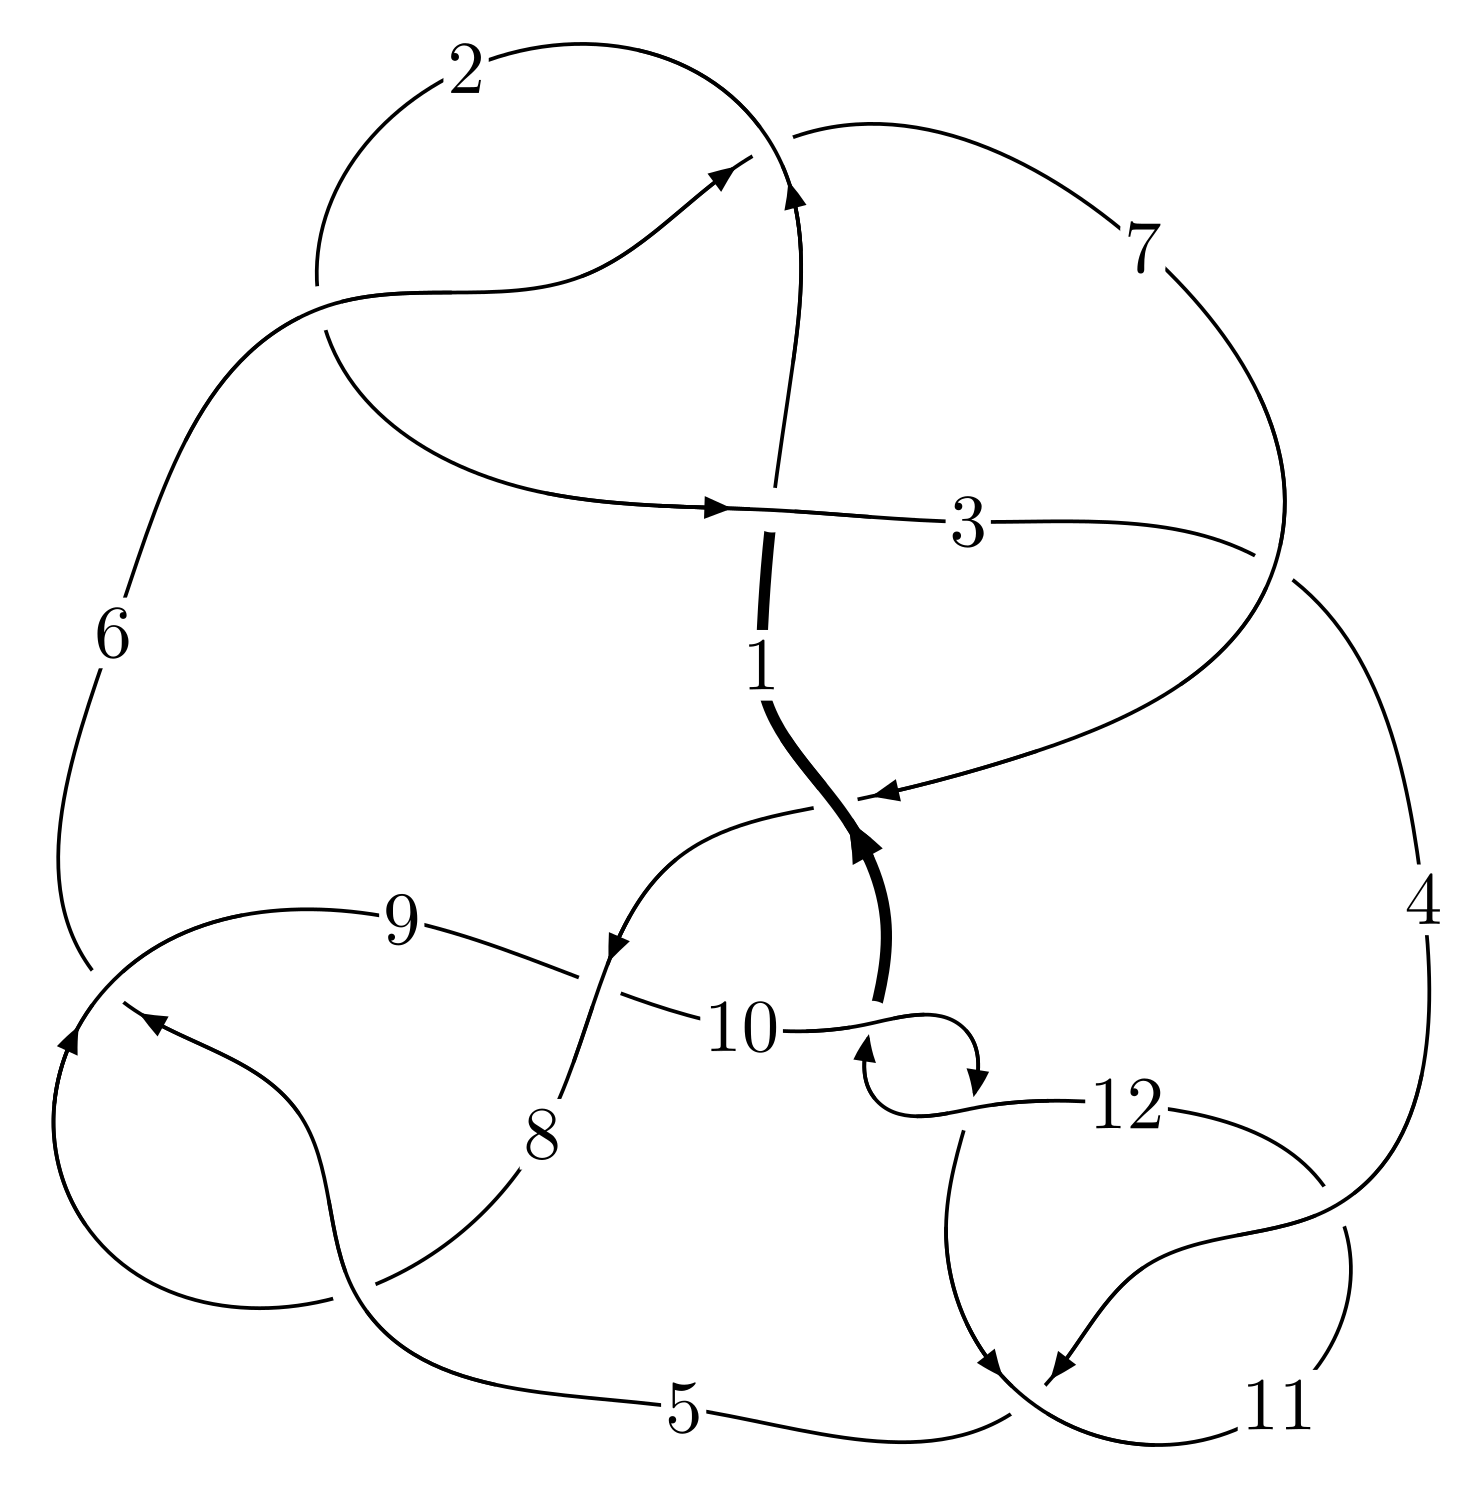
\includegraphics[width=112pt]{../../../GIT/diagram.site/Diagrams/png/1064_12a_0263.png}\\
\ \ \ A knot diagram\footnotemark}&
\allowdisplaybreaks
\textbf{Linearized knot diagam} \\
\cline{2-2}
 &
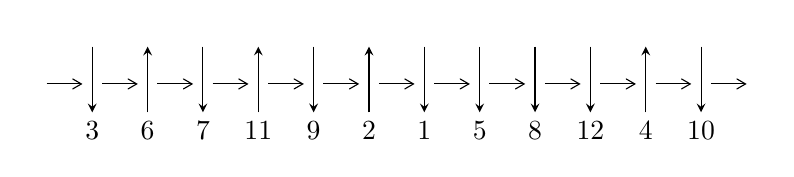
\begin{tikzpicture}[x=20pt, y=17pt]
	% nodes
	\node (C0) at (0, 0) {};
	\node (C1) at (1, 0) {};
	\node (C1U) at (1, +1) {};
	\node (C1D) at (1, -1) {3};

	\node (C2) at (2, 0) {};
	\node (C2U) at (2, +1) {};
	\node (C2D) at (2, -1) {6};

	\node (C3) at (3, 0) {};
	\node (C3U) at (3, +1) {};
	\node (C3D) at (3, -1) {7};

	\node (C4) at (4, 0) {};
	\node (C4U) at (4, +1) {};
	\node (C4D) at (4, -1) {11};

	\node (C5) at (5, 0) {};
	\node (C5U) at (5, +1) {};
	\node (C5D) at (5, -1) {9};

	\node (C6) at (6, 0) {};
	\node (C6U) at (6, +1) {};
	\node (C6D) at (6, -1) {2};

	\node (C7) at (7, 0) {};
	\node (C7U) at (7, +1) {};
	\node (C7D) at (7, -1) {1};

	\node (C8) at (8, 0) {};
	\node (C8U) at (8, +1) {};
	\node (C8D) at (8, -1) {5};

	\node (C9) at (9, 0) {};
	\node (C9U) at (9, +1) {};
	\node (C9D) at (9, -1) {8};

	\node (C10) at (10, 0) {};
	\node (C10U) at (10, +1) {};
	\node (C10D) at (10, -1) {12};

	\node (C11) at (11, 0) {};
	\node (C11U) at (11, +1) {};
	\node (C11D) at (11, -1) {4};

	\node (C12) at (12, 0) {};
	\node (C12U) at (12, +1) {};
	\node (C12D) at (12, -1) {10};
	\node (C13) at (13, 0) {};

	% arrows
	\draw[->,>={angle 60}]
	(C0) edge (C1) (C1) edge (C2) (C2) edge (C3) (C3) edge (C4) (C4) edge (C5) (C5) edge (C6) (C6) edge (C7) (C7) edge (C8) (C8) edge (C9) (C9) edge (C10) (C10) edge (C11) (C11) edge (C12) (C12) edge (C13) ;	\draw[->,>=stealth]
	(C1U) edge (C1D) (C2D) edge (C2U) (C3U) edge (C3D) (C4D) edge (C4U) (C5U) edge (C5D) (C6D) edge (C6U) (C7U) edge (C7D) (C8U) edge (C8D) (C9U) edge (C9D) (C10U) edge (C10D) (C11D) edge (C11U) (C12U) edge (C12D) ;
	\end{tikzpicture} \\
\hhline{~~} \\& 
\textbf{Solving Sequence} \\ \cline{2-2} 
 &
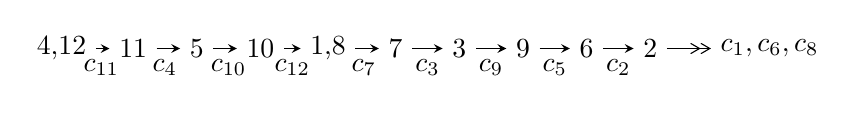
\begin{tikzpicture}[x=23pt, y=7pt]
	% node
	\node (A0) at (-1/8, 0) {4,12};
	\node (A1) at (1, 0) {11};
	\node (A2) at (2, 0) {5};
	\node (A3) at (3, 0) {10};
	\node (A4) at (65/16, 0) {1,8};
	\node (A5) at (41/8, 0) {7};
	\node (A6) at (49/8, 0) {3};
	\node (A7) at (57/8, 0) {9};
	\node (A8) at (65/8, 0) {6};
	\node (A9) at (73/8, 0) {2};
	\node (C1) at (1/2, -1) {$c_{11}$};
	\node (C2) at (3/2, -1) {$c_{4}$};
	\node (C3) at (5/2, -1) {$c_{10}$};
	\node (C4) at (7/2, -1) {$c_{12}$};
	\node (C5) at (37/8, -1) {$c_{7}$};
	\node (C6) at (45/8, -1) {$c_{3}$};
	\node (C7) at (53/8, -1) {$c_{9}$};
	\node (C8) at (61/8, -1) {$c_{5}$};
	\node (C9) at (69/8, -1) {$c_{2}$};
	\node (A10) at (11, 0) {$c_{1},c_{6},c_{8}$};

	% edge
	\draw[->,>=stealth]	
	(A0) edge (A1) (A1) edge (A2) (A2) edge (A3) (A3) edge (A4) (A4) edge (A5) (A5) edge (A6) (A6) edge (A7) (A7) edge (A8) (A8) edge (A9) ;
	\draw[->>,>={angle 60}]	
	(A9) edge (A10);
\end{tikzpicture} \\ 

\end{tabular} \\

\footnotetext{
The image of knot diagram is generated by the software ``\textbf{Draw programme}" developed by Andrew Bartholomew(\url{http://www.layer8.co.uk/maths/draw/index.htm\#Running-draw}), where we modified some parts for our purpose(\url{https://github.com/CATsTAILs/LinksPainter}).
}\phantom \\ \newline 
\centering \textbf{Ideals for irreducible components\footnotemark of $X_{\text{par}}$} 
 
\begin{align*}
I^u_{1}&=\langle 
2.01086\times10^{102} u^{114}+4.51397\times10^{102} u^{113}+\cdots+1.25045\times10^{102} b-1.17954\times10^{102},\\
\phantom{I^u_{1}}&\phantom{= \langle  }1.59104\times10^{102} u^{114}+1.66298\times10^{102} u^{113}+\cdots+1.25045\times10^{102} a+4.28857\times10^{102},\\
\phantom{I^u_{1}}&\phantom{= \langle  }u^{115}+2 u^{114}+\cdots+10 u-1\rangle \\
I^u_{2}&=\langle 
- a u+b- u+1,\;a^4+2 a^2 u+2 u-2,\;u^2- u+1\rangle \\
I^u_{3}&=\langle 
a u+b+u+1,\;a^3,\;u^2+u+1\rangle \\
\\
\end{align*}
\raggedright * 3 irreducible components of $\dim_{\mathbb{C}}=0$, with total 129 representations.\\
\footnotetext{All coefficients of polynomials are rational numbers. But the coefficients are sometimes approximated in decimal forms when there is not enough margin.}
\newpage
\renewcommand{\arraystretch}{1}
\centering \section*{I. $I^u_{1}= \langle 2.01\times10^{102} u^{114}+4.51\times10^{102} u^{113}+\cdots+1.25\times10^{102} b-1.18\times10^{102},\;1.59\times10^{102} u^{114}+1.66\times10^{102} u^{113}+\cdots+1.25\times10^{102} a+4.29\times10^{102},\;u^{115}+2 u^{114}+\cdots+10 u-1 \rangle$}
\flushleft \textbf{(i) Arc colorings}\\
\begin{tabular}{m{7pt} m{180pt} m{7pt} m{180pt} }
\flushright $a_{4}=$&$\begin{pmatrix}0\\u\end{pmatrix}$ \\
\flushright $a_{12}=$&$\begin{pmatrix}1\\0\end{pmatrix}$ \\
\flushright $a_{11}=$&$\begin{pmatrix}1\\u^2\end{pmatrix}$ \\
\flushright $a_{5}=$&$\begin{pmatrix}u\\u^3+u\end{pmatrix}$ \\
\flushright $a_{10}=$&$\begin{pmatrix}u^2+1\\u^2\end{pmatrix}$ \\
\flushright $a_{1}=$&$\begin{pmatrix}u^4+u^2+1\\u^4\end{pmatrix}$ \\
\flushright $a_{8}=$&$\begin{pmatrix}-1.27238 u^{114}-1.32991 u^{113}+\cdots+35.6015 u-3.42964\\-1.60812 u^{114}-3.60989 u^{113}+\cdots-18.7564 u+0.943297\end{pmatrix}$ \\
\flushright $a_{7}=$&$\begin{pmatrix}-1.62566 u^{114}-2.03980 u^{113}+\cdots+29.6716 u-3.74340\\-1.88288 u^{114}-3.94564 u^{113}+\cdots-15.7526 u+0.703551\end{pmatrix}$ \\
\flushright $a_{3}=$&$\begin{pmatrix}-0.271415 u^{114}-0.477569 u^{113}+\cdots-27.7578 u+7.77372\\-2.88361 u^{114}-3.20278 u^{113}+\cdots+9.23018 u-0.131897\end{pmatrix}$ \\
\flushright $a_{9}=$&$\begin{pmatrix}-1.84461 u^{114}-2.63457 u^{113}+\cdots+30.9998 u-2.90480\\-1.56401 u^{114}-3.81056 u^{113}+\cdots-22.3283 u+1.30793\end{pmatrix}$ \\
\flushright $a_{6}=$&$\begin{pmatrix}-0.0966470 u^{114}-0.878225 u^{113}+\cdots+55.5042 u-8.98908\\0.591189 u^{114}+0.769460 u^{113}+\cdots-4.98689 u-0.0147896\end{pmatrix}$ \\
\flushright $a_{2}=$&$\begin{pmatrix}-1.48684 u^{114}-2.97209 u^{113}+\cdots+56.2347 u+1.88650\\-3.04748 u^{114}-4.29788 u^{113}+\cdots+6.03056 u-0.234856\end{pmatrix}$\\&\end{tabular}
\flushleft \textbf{(ii) Obstruction class $= -1$}\\~\\
\flushleft \textbf{(iii) Cusp Shapes $= 0.560378 u^{114}-1.25164 u^{113}+\cdots+25.2254 u-10.9925$}\\~\\
\newpage\renewcommand{\arraystretch}{1}
\flushleft \textbf{(iv) u-Polynomials at the component}\newline \\
\begin{tabular}{m{50pt}|m{274pt}}
Crossings & \hspace{64pt}u-Polynomials at each crossing \\
\hline $$\begin{aligned}c_{1}\end{aligned}$$&$\begin{aligned}
&u^{115}+55 u^{114}+\cdots-80 u-16
\end{aligned}$\\
\hline $$\begin{aligned}c_{2},c_{6}\end{aligned}$$&$\begin{aligned}
&u^{115}- u^{114}+\cdots+4 u+4
\end{aligned}$\\
\hline $$\begin{aligned}c_{3}\end{aligned}$$&$\begin{aligned}
&u^{115}+u^{114}+\cdots+22772 u+8452
\end{aligned}$\\
\hline $$\begin{aligned}c_{4},c_{11}\end{aligned}$$&$\begin{aligned}
&u^{115}-2 u^{114}+\cdots+10 u+1
\end{aligned}$\\
\hline $$\begin{aligned}c_{5},c_{8}\end{aligned}$$&$\begin{aligned}
&u^{115}+3 u^{114}+\cdots+25 u+13
\end{aligned}$\\
\hline $$\begin{aligned}c_{7}\end{aligned}$$&$\begin{aligned}
&u^{115}-5 u^{114}+\cdots+185460 u+1006252
\end{aligned}$\\
\hline $$\begin{aligned}c_{9}\end{aligned}$$&$\begin{aligned}
&u^{115}+55 u^{114}+\cdots+2757 u+169
\end{aligned}$\\
\hline $$\begin{aligned}c_{10},c_{12}\end{aligned}$$&$\begin{aligned}
&u^{115}+38 u^{114}+\cdots-44 u-1
\end{aligned}$\\
\hline
\end{tabular}\\~\\
\newpage\renewcommand{\arraystretch}{1}
\flushleft \textbf{(v) Riley Polynomials at the component}\newline \\
\begin{tabular}{m{50pt}|m{274pt}}
Crossings & \hspace{64pt}Riley Polynomials at each crossing \\
\hline $$\begin{aligned}c_{1}\end{aligned}$$&$\begin{aligned}
&y^{115}+15 y^{114}+\cdots-5376 y-256
\end{aligned}$\\
\hline $$\begin{aligned}c_{2},c_{6}\end{aligned}$$&$\begin{aligned}
&y^{115}+55 y^{114}+\cdots-80 y-16
\end{aligned}$\\
\hline $$\begin{aligned}c_{3}\end{aligned}$$&$\begin{aligned}
&y^{115}-25 y^{114}+\cdots+3322126192 y-71436304
\end{aligned}$\\
\hline $$\begin{aligned}c_{4},c_{11}\end{aligned}$$&$\begin{aligned}
&y^{115}+38 y^{114}+\cdots-44 y-1
\end{aligned}$\\
\hline $$\begin{aligned}c_{5},c_{8}\end{aligned}$$&$\begin{aligned}
&y^{115}-55 y^{114}+\cdots+2757 y-169
\end{aligned}$\\
\hline $$\begin{aligned}c_{7}\end{aligned}$$&$\begin{aligned}
&y^{115}+35 y^{114}+\cdots-28479719212304 y-1012543087504
\end{aligned}$\\
\hline $$\begin{aligned}c_{9}\end{aligned}$$&$\begin{aligned}
&y^{115}+25 y^{114}+\cdots-632631 y-28561
\end{aligned}$\\
\hline $$\begin{aligned}c_{10},c_{12}\end{aligned}$$&$\begin{aligned}
&y^{115}+86 y^{114}+\cdots+2540 y-1
\end{aligned}$\\
\hline
\end{tabular}\\~\\
\newpage\flushleft \textbf{(vi) Complex Volumes and Cusp Shapes}
$$\begin{array}{c|c|c}  
\text{Solutions to }I^u_{1}& \I (\text{vol} + \sqrt{-1}CS) & \text{Cusp shape}\\
 \hline 
\begin{aligned}
u &= -0.317340 + 0.958509 I \\
a &= \phantom{-}0.386684 - 0.229998 I \\
b &= -0.590348 - 0.487723 I\end{aligned}
 & -0.35471 - 2.01312 I & \phantom{-0.000000 } 0 \\ \hline\begin{aligned}
u &= -0.317340 - 0.958509 I \\
a &= \phantom{-}0.386684 + 0.229998 I \\
b &= -0.590348 + 0.487723 I\end{aligned}
 & -0.35471 + 2.01312 I & \phantom{-0.000000 } 0 \\ \hline\begin{aligned}
u &= -0.402442 + 0.927578 I \\
a &= \phantom{-}0.283009 - 0.400198 I \\
b &= -0.524265 - 0.623213 I\end{aligned}
 & -0.33786 - 1.99475 I & \phantom{-0.000000 } 0 \\ \hline\begin{aligned}
u &= -0.402442 - 0.927578 I \\
a &= \phantom{-}0.283009 + 0.400198 I \\
b &= -0.524265 + 0.623213 I\end{aligned}
 & -0.33786 + 1.99475 I & \phantom{-0.000000 } 0 \\ \hline\begin{aligned}
u &= \phantom{-}0.128604 + 0.973698 I \\
a &= \phantom{-}0.469012 + 0.081766 I \\
b &= -0.637499 + 0.192073 I\end{aligned}
 & -4.02849 - 0.46501 I & \phantom{-0.000000 } 0 \\ \hline\begin{aligned}
u &= \phantom{-}0.128604 - 0.973698 I \\
a &= \phantom{-}0.469012 - 0.081766 I \\
b &= -0.637499 - 0.192073 I\end{aligned}
 & -4.02849 + 0.46501 I & \phantom{-0.000000 } 0 \\ \hline\begin{aligned}
u &= -0.026955 + 0.979717 I \\
a &= -1.204110 - 0.681289 I \\
b &= \phantom{-}0.231698 - 1.130490 I\end{aligned}
 & -7.59317 - 3.77195 I & \phantom{-0.000000 } 0 \\ \hline\begin{aligned}
u &= -0.026955 - 0.979717 I \\
a &= -1.204110 + 0.681289 I \\
b &= \phantom{-}0.231698 + 1.130490 I\end{aligned}
 & -7.59317 + 3.77195 I & \phantom{-0.000000 } 0 \\ \hline\begin{aligned}
u &= \phantom{-}0.694392 + 0.747476 I \\
a &= -1.28801 + 2.18792 I \\
b &= -2.54657 + 0.36171 I\end{aligned}
 & -2.72628 - 3.43267 I & \phantom{-0.000000 } 0 \\ \hline\begin{aligned}
u &= \phantom{-}0.694392 - 0.747476 I \\
a &= -1.28801 - 2.18792 I \\
b &= -2.54657 - 0.36171 I\end{aligned}
 & -2.72628 + 3.43267 I & \phantom{-0.000000 } 0\\
 \hline 
 \end{array}$$\newpage$$\begin{array}{c|c|c}  
\text{Solutions to }I^u_{1}& \I (\text{vol} + \sqrt{-1}CS) & \text{Cusp shape}\\
 \hline 
\begin{aligned}
u &= \phantom{-}0.666498 + 0.806418 I \\
a &= -0.70376 + 2.31939 I \\
b &= -2.30466 + 0.80638 I\end{aligned}
 & -2.41073 + 4.83529 I & \phantom{-0.000000 } 0 \\ \hline\begin{aligned}
u &= \phantom{-}0.666498 - 0.806418 I \\
a &= -0.70376 - 2.31939 I \\
b &= -2.30466 - 0.80638 I\end{aligned}
 & -2.41073 - 4.83529 I & \phantom{-0.000000 } 0 \\ \hline\begin{aligned}
u &= -0.708294 + 0.793455 I \\
a &= -0.96316 - 2.03713 I \\
b &= -2.27747 - 0.46831 I\end{aligned}
 & \phantom{-}0.797868 - 0.556912 I & \phantom{-0.000000 } 0 \\ \hline\begin{aligned}
u &= -0.708294 - 0.793455 I \\
a &= -0.96316 + 2.03713 I \\
b &= -2.27747 + 0.46831 I\end{aligned}
 & \phantom{-}0.797868 + 0.556912 I & \phantom{-0.000000 } 0 \\ \hline\begin{aligned}
u &= -0.724070 + 0.786554 I \\
a &= \phantom{-}0.205092 + 0.138209 I \\
b &= -0.442316 - 1.079350 I\end{aligned}
 & -1.61875 + 2.86367 I & \phantom{-0.000000 } 0 \\ \hline\begin{aligned}
u &= -0.724070 - 0.786554 I \\
a &= \phantom{-}0.205092 - 0.138209 I \\
b &= -0.442316 + 1.079350 I\end{aligned}
 & -1.61875 - 2.86367 I & \phantom{-0.000000 } 0 \\ \hline\begin{aligned}
u &= -0.827334 + 0.679561 I \\
a &= -1.50772 - 1.47621 I \\
b &= -2.34589 + 0.07969 I\end{aligned}
 & \phantom{-}0.02962 + 3.95638 I & \phantom{-0.000000 } 0 \\ \hline\begin{aligned}
u &= -0.827334 - 0.679561 I \\
a &= -1.50772 + 1.47621 I \\
b &= -2.34589 - 0.07969 I\end{aligned}
 & \phantom{-}0.02962 - 3.95638 I & \phantom{-0.000000 } 0 \\ \hline\begin{aligned}
u &= \phantom{-}0.258721 + 1.039580 I \\
a &= \phantom{-}0.382183 + 0.132670 I \\
b &= -0.728654 + 0.401051 I\end{aligned}
 & -2.42367 + 6.60021 I & \phantom{-0.000000 } 0 \\ \hline\begin{aligned}
u &= \phantom{-}0.258721 - 1.039580 I \\
a &= \phantom{-}0.382183 - 0.132670 I \\
b &= -0.728654 - 0.401051 I\end{aligned}
 & -2.42367 - 6.60021 I & \phantom{-0.000000 } 0\\
 \hline 
 \end{array}$$\newpage$$\begin{array}{c|c|c}  
\text{Solutions to }I^u_{1}& \I (\text{vol} + \sqrt{-1}CS) & \text{Cusp shape}\\
 \hline 
\begin{aligned}
u &= -0.626056 + 0.680132 I \\
a &= \phantom{-}0.144981 + 0.252917 I \\
b &= -0.371864 - 0.971815 I\end{aligned}
 & -3.17538 - 3.53458 I & \phantom{-0.000000 } 0 \\ \hline\begin{aligned}
u &= -0.626056 - 0.680132 I \\
a &= \phantom{-}0.144981 - 0.252917 I \\
b &= -0.371864 + 0.971815 I\end{aligned}
 & -3.17538 + 3.53458 I & \phantom{-0.000000 } 0 \\ \hline\begin{aligned}
u &= \phantom{-}0.460669 + 0.974433 I \\
a &= -0.039605 + 0.716668 I \\
b &= -0.556193 + 0.580174 I\end{aligned}
 & -2.21464 + 5.95174 I & \phantom{-0.000000 } 0 \\ \hline\begin{aligned}
u &= \phantom{-}0.460669 - 0.974433 I \\
a &= -0.039605 - 0.716668 I \\
b &= -0.556193 - 0.580174 I\end{aligned}
 & -2.21464 - 5.95174 I & \phantom{-0.000000 } 0 \\ \hline\begin{aligned}
u &= \phantom{-}0.698183 + 0.826164 I \\
a &= \phantom{-}0.185654 - 0.111531 I \\
b &= -0.486437 + 1.059710 I\end{aligned}
 & \phantom{-}0.17908 + 1.79961 I & \phantom{-0.000000 } 0 \\ \hline\begin{aligned}
u &= \phantom{-}0.698183 - 0.826164 I \\
a &= \phantom{-}0.185654 + 0.111531 I \\
b &= -0.486437 - 1.059710 I\end{aligned}
 & \phantom{-}0.17908 - 1.79961 I & \phantom{-0.000000 } 0 \\ \hline\begin{aligned}
u &= \phantom{-}0.323763 + 1.038830 I \\
a &= -0.465298 + 0.598826 I \\
b &= -0.216214 + 0.536876 I\end{aligned}
 & -2.15583 + 0.04366 I & \phantom{-0.000000 } 0 \\ \hline\begin{aligned}
u &= \phantom{-}0.323763 - 1.038830 I \\
a &= -0.465298 - 0.598826 I \\
b &= -0.216214 - 0.536876 I\end{aligned}
 & -2.15583 - 0.04366 I & \phantom{-0.000000 } 0 \\ \hline\begin{aligned}
u &= \phantom{-}0.031176 + 0.910871 I \\
a &= -1.54113 - 0.58458 I \\
b &= \phantom{-}0.11802 - 1.42138 I\end{aligned}
 & -6.42366 + 3.97352 I & \phantom{-0.000000 } 0 \\ \hline\begin{aligned}
u &= \phantom{-}0.031176 - 0.910871 I \\
a &= -1.54113 + 0.58458 I \\
b &= \phantom{-}0.11802 + 1.42138 I\end{aligned}
 & -6.42366 - 3.97352 I & \phantom{-0.000000 } 0\\
 \hline 
 \end{array}$$\newpage$$\begin{array}{c|c|c}  
\text{Solutions to }I^u_{1}& \I (\text{vol} + \sqrt{-1}CS) & \text{Cusp shape}\\
 \hline 
\begin{aligned}
u &= -0.778984 + 0.761257 I \\
a &= \phantom{-}1.41887 + 0.08520 I \\
b &= \phantom{-}1.38202 - 0.77443 I\end{aligned}
 & \phantom{-}1.81812 - 1.36653 I & \phantom{-0.000000 } 0 \\ \hline\begin{aligned}
u &= -0.778984 - 0.761257 I \\
a &= \phantom{-}1.41887 - 0.08520 I \\
b &= \phantom{-}1.38202 + 0.77443 I\end{aligned}
 & \phantom{-}1.81812 + 1.36653 I & \phantom{-0.000000 } 0 \\ \hline\begin{aligned}
u &= -0.248236 + 1.061000 I \\
a &= -0.616685 - 0.634563 I \\
b &= -0.040821 - 0.575935 I\end{aligned}
 & -0.96649 - 4.49766 I & \phantom{-0.000000 } 0 \\ \hline\begin{aligned}
u &= -0.248236 - 1.061000 I \\
a &= -0.616685 + 0.634563 I \\
b &= -0.040821 + 0.575935 I\end{aligned}
 & -0.96649 + 4.49766 I & \phantom{-0.000000 } 0 \\ \hline\begin{aligned}
u &= \phantom{-}0.134648 + 1.088300 I \\
a &= -0.805339 + 0.756823 I \\
b &= \phantom{-}0.233553 + 0.683296 I\end{aligned}
 & -6.57020 + 3.75115 I & \phantom{-0.000000 } 0 \\ \hline\begin{aligned}
u &= \phantom{-}0.134648 - 1.088300 I \\
a &= -0.805339 - 0.756823 I \\
b &= \phantom{-}0.233553 - 0.683296 I\end{aligned}
 & -6.57020 - 3.75115 I & \phantom{-0.000000 } 0 \\ \hline\begin{aligned}
u &= -0.871760 + 0.670108 I \\
a &= -1.49364 - 1.33520 I \\
b &= -2.31543 + 0.13900 I\end{aligned}
 & \phantom{-}2.73154 + 11.80690 I & \phantom{-0.000000 } 0 \\ \hline\begin{aligned}
u &= -0.871760 - 0.670108 I \\
a &= -1.49364 + 1.33520 I \\
b &= -2.31543 - 0.13900 I\end{aligned}
 & \phantom{-}2.73154 - 11.80690 I & \phantom{-0.000000 } 0 \\ \hline\begin{aligned}
u &= \phantom{-}0.026040 + 0.898962 I \\
a &= -1.35487 + 0.42745 I \\
b &= \phantom{-}0.011317 + 1.254750 I\end{aligned}
 & -3.84623 + 0.56310 I & \phantom{-0.000000 } 0 \\ \hline\begin{aligned}
u &= \phantom{-}0.026040 - 0.898962 I \\
a &= -1.35487 - 0.42745 I \\
b &= \phantom{-}0.011317 - 1.254750 I\end{aligned}
 & -3.84623 - 0.56310 I & \phantom{-0.000000 } 0\\
 \hline 
 \end{array}$$\newpage$$\begin{array}{c|c|c}  
\text{Solutions to }I^u_{1}& \I (\text{vol} + \sqrt{-1}CS) & \text{Cusp shape}\\
 \hline 
\begin{aligned}
u &= \phantom{-}0.864664 + 0.686181 I \\
a &= -1.45479 + 1.36848 I \\
b &= -2.30195 - 0.11899 I\end{aligned}
 & \phantom{-}4.98326 - 6.60319 I & \phantom{-0.000000 } 0 \\ \hline\begin{aligned}
u &= \phantom{-}0.864664 - 0.686181 I \\
a &= -1.45479 - 1.36848 I \\
b &= -2.30195 + 0.11899 I\end{aligned}
 & \phantom{-}4.98326 + 6.60319 I & \phantom{-0.000000 } 0 \\ \hline\begin{aligned}
u &= -0.850826 + 0.737880 I \\
a &= \phantom{-}1.261740 + 0.172476 I \\
b &= \phantom{-}1.46412 - 0.48516 I\end{aligned}
 & \phantom{-}4.83005 + 5.88847 I & \phantom{-0.000000 } 0 \\ \hline\begin{aligned}
u &= -0.850826 - 0.737880 I \\
a &= \phantom{-}1.261740 - 0.172476 I \\
b &= \phantom{-}1.46412 + 0.48516 I\end{aligned}
 & \phantom{-}4.83005 - 5.88847 I & \phantom{-0.000000 } 0 \\ \hline\begin{aligned}
u &= \phantom{-}0.854308 + 0.736997 I \\
a &= -1.30960 + 1.42441 I \\
b &= -2.23295 - 0.06543 I\end{aligned}
 & \phantom{-}6.34337 - 3.89444 I & \phantom{-0.000000 } 0 \\ \hline\begin{aligned}
u &= \phantom{-}0.854308 - 0.736997 I \\
a &= -1.30960 - 1.42441 I \\
b &= -2.23295 + 0.06543 I\end{aligned}
 & \phantom{-}6.34337 + 3.89444 I & \phantom{-0.000000 } 0 \\ \hline\begin{aligned}
u &= -0.181265 + 1.113750 I \\
a &= -0.706748 - 0.756843 I \\
b &= \phantom{-}0.170293 - 0.556044 I\end{aligned}
 & -2.14972 - 6.38550 I & \phantom{-0.000000 } 0 \\ \hline\begin{aligned}
u &= -0.181265 - 1.113750 I \\
a &= -0.706748 + 0.756843 I \\
b &= \phantom{-}0.170293 + 0.556044 I\end{aligned}
 & -2.14972 + 6.38550 I & \phantom{-0.000000 } 0 \\ \hline\begin{aligned}
u &= \phantom{-}0.841809 + 0.760377 I \\
a &= \phantom{-}1.306360 - 0.196562 I \\
b &= \phantom{-}1.51714 + 0.55395 I\end{aligned}
 & \phantom{-}6.84731 - 0.71770 I & \phantom{-0.000000 } 0 \\ \hline\begin{aligned}
u &= \phantom{-}0.841809 - 0.760377 I \\
a &= \phantom{-}1.306360 + 0.196562 I \\
b &= \phantom{-}1.51714 - 0.55395 I\end{aligned}
 & \phantom{-}6.84731 + 0.71770 I & \phantom{-0.000000 } 0\\
 \hline 
 \end{array}$$\newpage$$\begin{array}{c|c|c}  
\text{Solutions to }I^u_{1}& \I (\text{vol} + \sqrt{-1}CS) & \text{Cusp shape}\\
 \hline 
\begin{aligned}
u &= \phantom{-}0.676120 + 0.916879 I \\
a &= \phantom{-}2.43848 - 0.65220 I \\
b &= \phantom{-}2.43582 + 1.75520 I\end{aligned}
 & -2.75576 + 0.37527 I & \phantom{-0.000000 } 0 \\ \hline\begin{aligned}
u &= \phantom{-}0.676120 - 0.916879 I \\
a &= \phantom{-}2.43848 + 0.65220 I \\
b &= \phantom{-}2.43582 - 1.75520 I\end{aligned}
 & -2.75576 - 0.37527 I & \phantom{-0.000000 } 0 \\ \hline\begin{aligned}
u &= -0.845635 + 0.765410 I \\
a &= -1.22224 - 1.45135 I \\
b &= -2.18300 + 0.02983 I\end{aligned}
 & \phantom{-}5.32733 - 1.21844 I & \phantom{-0.000000 } 0 \\ \hline\begin{aligned}
u &= -0.845635 - 0.765410 I \\
a &= -1.22224 + 1.45135 I \\
b &= -2.18300 - 0.02983 I\end{aligned}
 & \phantom{-}5.32733 + 1.21844 I & \phantom{-0.000000 } 0 \\ \hline\begin{aligned}
u &= -0.461959 + 1.044150 I \\
a &= \phantom{-}0.223137 - 0.119182 I \\
b &= -0.732537 - 0.736053 I\end{aligned}
 & -0.478894 - 0.657716 I & \phantom{-0.000000 } 0 \\ \hline\begin{aligned}
u &= -0.461959 - 1.044150 I \\
a &= \phantom{-}0.223137 + 0.119182 I \\
b &= -0.732537 + 0.736053 I\end{aligned}
 & -0.478894 + 0.657716 I & \phantom{-0.000000 } 0 \\ \hline\begin{aligned}
u &= \phantom{-}0.693639 + 0.909576 I \\
a &= \phantom{-}0.193363 - 0.058251 I \\
b &= -0.577465 + 1.062100 I\end{aligned}
 & -0.08212 + 3.55372 I & \phantom{-0.000000 } 0 \\ \hline\begin{aligned}
u &= \phantom{-}0.693639 - 0.909576 I \\
a &= \phantom{-}0.193363 + 0.058251 I \\
b &= -0.577465 - 1.062100 I\end{aligned}
 & -0.08212 - 3.55372 I & \phantom{-0.000000 } 0 \\ \hline\begin{aligned}
u &= \phantom{-}0.168392 + 1.135500 I \\
a &= -0.708913 + 0.798541 I \\
b &= \phantom{-}0.230419 + 0.525876 I\end{aligned}
 & -4.41133 + 11.33980 I & \phantom{-0.000000 } 0 \\ \hline\begin{aligned}
u &= \phantom{-}0.168392 - 1.135500 I \\
a &= -0.708913 - 0.798541 I \\
b &= \phantom{-}0.230419 - 0.525876 I\end{aligned}
 & -4.41133 - 11.33980 I & \phantom{-0.000000 } 0\\
 \hline 
 \end{array}$$\newpage$$\begin{array}{c|c|c}  
\text{Solutions to }I^u_{1}& \I (\text{vol} + \sqrt{-1}CS) & \text{Cusp shape}\\
 \hline 
\begin{aligned}
u &= -0.638048 + 0.960706 I \\
a &= \phantom{-}0.180951 + 0.014452 I \\
b &= -0.638750 - 0.996248 I\end{aligned}
 & -4.00322 - 1.44759 I & \phantom{-0.000000 } 0 \\ \hline\begin{aligned}
u &= -0.638048 - 0.960706 I \\
a &= \phantom{-}0.180951 - 0.014452 I \\
b &= -0.638750 + 0.996248 I\end{aligned}
 & -4.00322 + 1.44759 I & \phantom{-0.000000 } 0 \\ \hline\begin{aligned}
u &= \phantom{-}0.540566 + 1.025900 I \\
a &= \phantom{-}0.191456 + 0.062867 I \\
b &= -0.715366 + 0.859306 I\end{aligned}
 & -4.17186 + 2.86985 I & \phantom{-0.000000 } 0 \\ \hline\begin{aligned}
u &= \phantom{-}0.540566 - 1.025900 I \\
a &= \phantom{-}0.191456 - 0.062867 I \\
b &= -0.715366 - 0.859306 I\end{aligned}
 & -4.17186 - 2.86985 I & \phantom{-0.000000 } 0 \\ \hline\begin{aligned}
u &= -0.699803 + 0.930419 I \\
a &= \phantom{-}2.16993 + 0.76694 I \\
b &= \phantom{-}2.45168 - 1.44491 I\end{aligned}
 & \phantom{-}0.37777 - 4.85201 I & \phantom{-0.000000 } 0 \\ \hline\begin{aligned}
u &= -0.699803 - 0.930419 I \\
a &= \phantom{-}2.16993 - 0.76694 I \\
b &= \phantom{-}2.45168 + 1.44491 I\end{aligned}
 & \phantom{-}0.37777 + 4.85201 I & \phantom{-0.000000 } 0 \\ \hline\begin{aligned}
u &= \phantom{-}0.832444 + 0.818924 I \\
a &= \phantom{-}1.40275 - 0.30782 I \\
b &= \phantom{-}1.71169 + 0.67772 I\end{aligned}
 & \phantom{-}7.54796 + 2.04605 I & \phantom{-0.000000 } 0 \\ \hline\begin{aligned}
u &= \phantom{-}0.832444 - 0.818924 I \\
a &= \phantom{-}1.40275 + 0.30782 I \\
b &= \phantom{-}1.71169 - 0.67772 I\end{aligned}
 & \phantom{-}7.54796 - 2.04605 I & \phantom{-0.000000 } 0 \\ \hline\begin{aligned}
u &= -0.705536 + 0.937868 I \\
a &= \phantom{-}0.205471 + 0.046417 I \\
b &= -0.609989 - 1.077930 I\end{aligned}
 & -2.08271 - 8.33515 I & \phantom{-0.000000 } 0 \\ \hline\begin{aligned}
u &= -0.705536 - 0.937868 I \\
a &= \phantom{-}0.205471 - 0.046417 I \\
b &= -0.609989 + 1.077930 I\end{aligned}
 & -2.08271 + 8.33515 I & \phantom{-0.000000 } 0\\
 \hline 
 \end{array}$$\newpage$$\begin{array}{c|c|c}  
\text{Solutions to }I^u_{1}& \I (\text{vol} + \sqrt{-1}CS) & \text{Cusp shape}\\
 \hline 
\begin{aligned}
u &= \phantom{-}0.685259 + 0.956395 I \\
a &= \phantom{-}2.22212 - 1.05324 I \\
b &= \phantom{-}2.74734 + 1.39961 I\end{aligned}
 & -3.36219 + 8.76415 I & \phantom{-0.000000 } 0 \\ \hline\begin{aligned}
u &= \phantom{-}0.685259 - 0.956395 I \\
a &= \phantom{-}2.22212 + 1.05324 I \\
b &= \phantom{-}2.74734 - 1.39961 I\end{aligned}
 & -3.36219 - 8.76415 I & \phantom{-0.000000 } 0 \\ \hline\begin{aligned}
u &= \phantom{-}0.484616 + 1.074600 I \\
a &= \phantom{-}0.232791 + 0.092293 I \\
b &= -0.782883 + 0.769243 I\end{aligned}
 & -2.48486 - 4.00622 I & \phantom{-0.000000 } 0 \\ \hline\begin{aligned}
u &= \phantom{-}0.484616 - 1.074600 I \\
a &= \phantom{-}0.232791 - 0.092293 I \\
b &= -0.782883 - 0.769243 I\end{aligned}
 & -2.48486 + 4.00622 I & \phantom{-0.000000 } 0 \\ \hline\begin{aligned}
u &= -0.829054 + 0.847083 I \\
a &= \phantom{-}1.44147 + 0.38054 I \\
b &= \phantom{-}1.82162 - 0.71939 I\end{aligned}
 & \phantom{-}6.17057 - 7.18545 I & \phantom{-0.000000 } 0 \\ \hline\begin{aligned}
u &= -0.829054 - 0.847083 I \\
a &= \phantom{-}1.44147 - 0.38054 I \\
b &= \phantom{-}1.82162 + 0.71939 I\end{aligned}
 & \phantom{-}6.17057 + 7.18545 I & \phantom{-0.000000 } 0 \\ \hline\begin{aligned}
u &= \phantom{-}0.768739 + 0.209948 I \\
a &= \phantom{-}0.617926 - 0.322861 I \\
b &= \phantom{-}0.095937 + 0.776814 I\end{aligned}
 & \phantom{-}0.12317 + 8.45001 I & -2.28233 - 8.06437 I \\ \hline\begin{aligned}
u &= \phantom{-}0.768739 - 0.209948 I \\
a &= \phantom{-}0.617926 + 0.322861 I \\
b &= \phantom{-}0.095937 - 0.776814 I\end{aligned}
 & \phantom{-}0.12317 - 8.45001 I & -2.28233 + 8.06437 I \\ \hline\begin{aligned}
u &= -0.730015 + 0.969514 I \\
a &= -0.52972 - 1.34051 I \\
b &= -1.46590 - 0.19585 I\end{aligned}
 & \phantom{-}1.17851 - 4.34244 I & \phantom{-0.000000 } 0 \\ \hline\begin{aligned}
u &= -0.730015 - 0.969514 I \\
a &= -0.52972 + 1.34051 I \\
b &= -1.46590 + 0.19585 I\end{aligned}
 & \phantom{-}1.17851 + 4.34244 I & \phantom{-0.000000 } 0\\
 \hline 
 \end{array}$$\newpage$$\begin{array}{c|c|c}  
\text{Solutions to }I^u_{1}& \I (\text{vol} + \sqrt{-1}CS) & \text{Cusp shape}\\
 \hline 
\begin{aligned}
u &= -0.798015 + 0.923550 I \\
a &= -0.74712 - 1.37409 I \\
b &= -1.72957 - 0.06860 I\end{aligned}
 & \phantom{-}5.93008 + 1.11957 I & \phantom{-0.000000 } 0 \\ \hline\begin{aligned}
u &= -0.798015 - 0.923550 I \\
a &= -0.74712 + 1.37409 I \\
b &= -1.72957 + 0.06860 I\end{aligned}
 & \phantom{-}5.93008 - 1.11957 I & \phantom{-0.000000 } 0 \\ \hline\begin{aligned}
u &= \phantom{-}0.786185 + 0.947127 I \\
a &= -0.68717 + 1.34227 I \\
b &= -1.64246 + 0.07053 I\end{aligned}
 & \phantom{-}7.14895 + 3.99371 I & \phantom{-0.000000 } 0 \\ \hline\begin{aligned}
u &= \phantom{-}0.786185 - 0.947127 I \\
a &= -0.68717 - 1.34227 I \\
b &= -1.64246 - 0.07053 I\end{aligned}
 & \phantom{-}7.14895 - 3.99371 I & \phantom{-0.000000 } 0 \\ \hline\begin{aligned}
u &= -0.738485 + 0.172014 I \\
a &= \phantom{-}0.660657 + 0.338783 I \\
b &= \phantom{-}0.102769 - 0.712483 I\end{aligned}
 & \phantom{-}2.13287 - 3.50579 I & \phantom{-}1.21650 + 3.83192 I \\ \hline\begin{aligned}
u &= -0.738485 - 0.172014 I \\
a &= \phantom{-}0.660657 - 0.338783 I \\
b &= \phantom{-}0.102769 + 0.712483 I\end{aligned}
 & \phantom{-}2.13287 + 3.50579 I & \phantom{-}1.21650 - 3.83192 I \\ \hline\begin{aligned}
u &= \phantom{-}0.231126 + 0.716714 I \\
a &= -0.721833 - 0.339395 I \\
b &= -0.401428 + 0.953330 I\end{aligned}
 & -2.30795 + 0.81433 I & -8.21026 + 1.09447 I \\ \hline\begin{aligned}
u &= \phantom{-}0.231126 - 0.716714 I \\
a &= -0.721833 + 0.339395 I \\
b &= -0.401428 - 0.953330 I\end{aligned}
 & -2.30795 - 0.81433 I & -8.21026 - 1.09447 I \\ \hline\begin{aligned}
u &= \phantom{-}0.764333 + 0.988730 I \\
a &= -0.599704 + 1.274690 I \\
b &= -1.48584 + 0.05708 I\end{aligned}
 & \phantom{-}6.14132 + 6.71356 I & \phantom{-0.000000 } 0 \\ \hline\begin{aligned}
u &= \phantom{-}0.764333 - 0.988730 I \\
a &= -0.599704 - 1.274690 I \\
b &= -1.48584 - 0.05708 I\end{aligned}
 & \phantom{-}6.14132 - 6.71356 I & \phantom{-0.000000 } 0\\
 \hline 
 \end{array}$$\newpage$$\begin{array}{c|c|c}  
\text{Solutions to }I^u_{1}& \I (\text{vol} + \sqrt{-1}CS) & \text{Cusp shape}\\
 \hline 
\begin{aligned}
u &= -0.769206 + 0.986480 I \\
a &= \phantom{-}1.60436 + 0.94967 I \\
b &= \phantom{-}2.48983 - 0.83752 I\end{aligned}
 & \phantom{-}4.64360 - 4.80354 I & \phantom{-0.000000 } 0 \\ \hline\begin{aligned}
u &= -0.769206 - 0.986480 I \\
a &= \phantom{-}1.60436 - 0.94967 I \\
b &= \phantom{-}2.48983 + 0.83752 I\end{aligned}
 & \phantom{-}4.64360 + 4.80354 I & \phantom{-0.000000 } 0 \\ \hline\begin{aligned}
u &= -0.726511 + 1.024300 I \\
a &= \phantom{-}1.63961 + 1.25436 I \\
b &= \phantom{-}2.76929 - 0.81489 I\end{aligned}
 & -1.01875 - 9.78161 I & \phantom{-0.000000 } 0 \\ \hline\begin{aligned}
u &= -0.726511 - 1.024300 I \\
a &= \phantom{-}1.63961 - 1.25436 I \\
b &= \phantom{-}2.76929 + 0.81489 I\end{aligned}
 & -1.01875 + 9.78161 I & \phantom{-0.000000 } 0 \\ \hline\begin{aligned}
u &= -0.759815 + 1.004580 I \\
a &= -0.581263 - 1.244870 I \\
b &= -1.43530 - 0.03633 I\end{aligned}
 & \phantom{-}4.00721 - 11.89380 I & \phantom{-0.000000 } 0 \\ \hline\begin{aligned}
u &= -0.759815 - 1.004580 I \\
a &= -0.581263 + 1.244870 I \\
b &= -1.43530 + 0.03633 I\end{aligned}
 & \phantom{-}4.00721 + 11.89380 I & \phantom{-0.000000 } 0 \\ \hline\begin{aligned}
u &= \phantom{-}0.762064 + 1.006710 I \\
a &= \phantom{-}1.57450 - 1.05010 I \\
b &= \phantom{-}2.57894 + 0.79504 I\end{aligned}
 & \phantom{-}5.51171 + 9.91734 I & \phantom{-0.000000 } 0 \\ \hline\begin{aligned}
u &= \phantom{-}0.762064 - 1.006710 I \\
a &= \phantom{-}1.57450 + 1.05010 I \\
b &= \phantom{-}2.57894 - 0.79504 I\end{aligned}
 & \phantom{-}5.51171 - 9.91734 I & \phantom{-0.000000 } 0 \\ \hline\begin{aligned}
u &= \phantom{-}0.744393 + 1.035660 I \\
a &= \phantom{-}1.52987 - 1.21436 I \\
b &= \phantom{-}2.71444 + 0.73036 I\end{aligned}
 & \phantom{-}3.90897 + 12.59190 I & \phantom{-0.000000 } 0 \\ \hline\begin{aligned}
u &= \phantom{-}0.744393 - 1.035660 I \\
a &= \phantom{-}1.52987 + 1.21436 I \\
b &= \phantom{-}2.71444 - 0.73036 I\end{aligned}
 & \phantom{-}3.90897 - 12.59190 I & \phantom{-0.000000 } 0\\
 \hline 
 \end{array}$$\newpage$$\begin{array}{c|c|c}  
\text{Solutions to }I^u_{1}& \I (\text{vol} + \sqrt{-1}CS) & \text{Cusp shape}\\
 \hline 
\begin{aligned}
u &= -0.740577 + 1.045390 I \\
a &= \phantom{-}1.50029 + 1.25885 I \\
b &= \phantom{-}2.74585 - 0.69836 I\end{aligned}
 & \phantom{-}1.5783 - 17.8002 I & \phantom{-0.000000 } 0 \\ \hline\begin{aligned}
u &= -0.740577 - 1.045390 I \\
a &= \phantom{-}1.50029 - 1.25885 I \\
b &= \phantom{-}2.74585 + 0.69836 I\end{aligned}
 & \phantom{-}1.5783 + 17.8002 I & \phantom{-0.000000 } 0 \\ \hline\begin{aligned}
u &= -0.404828 + 0.591987 I \\
a &= \phantom{-}0.879232 - 0.270418 I \\
b &= \phantom{-}0.067261 - 0.367460 I\end{aligned}
 & \phantom{-}0.44130 - 1.44965 I & \phantom{-}1.24412 + 4.77904 I \\ \hline\begin{aligned}
u &= -0.404828 - 0.591987 I \\
a &= \phantom{-}0.879232 + 0.270418 I \\
b &= \phantom{-}0.067261 + 0.367460 I\end{aligned}
 & \phantom{-}0.44130 + 1.44965 I & \phantom{-}1.24412 - 4.77904 I \\ \hline\begin{aligned}
u &= \phantom{-}0.712733 + 0.030064 I \\
a &= \phantom{-}0.819187 + 0.256273 I \\
b &= \phantom{-}0.269915 - 0.478438 I\end{aligned}
 & \phantom{-}1.05289 + 3.41428 I & -0.14497 - 2.59163 I \\ \hline\begin{aligned}
u &= \phantom{-}0.712733 - 0.030064 I \\
a &= \phantom{-}0.819187 - 0.256273 I \\
b &= \phantom{-}0.269915 + 0.478438 I\end{aligned}
 & \phantom{-}1.05289 - 3.41428 I & -0.14497 + 2.59163 I \\ \hline\begin{aligned}
u &= -0.703794 + 0.045782 I \\
a &= \phantom{-}0.779121 + 0.305557 I \\
b &= \phantom{-}0.187077 - 0.551290 I\end{aligned}
 & \phantom{-}2.62952 - 1.36952 I & \phantom{-}2.63173 + 3.11648 I \\ \hline\begin{aligned}
u &= -0.703794 - 0.045782 I \\
a &= \phantom{-}0.779121 - 0.305557 I \\
b &= \phantom{-}0.187077 + 0.551290 I\end{aligned}
 & \phantom{-}2.62952 + 1.36952 I & \phantom{-}2.63173 - 3.11648 I \\ \hline\begin{aligned}
u &= \phantom{-}0.627772 + 0.271576 I \\
a &= \phantom{-}0.580861 - 0.493039 I \\
b &= -0.089198 + 0.712756 I\end{aligned}
 & -2.24966 + 1.49423 I & -6.29073 - 2.74212 I \\ \hline\begin{aligned}
u &= \phantom{-}0.627772 - 0.271576 I \\
a &= \phantom{-}0.580861 + 0.493039 I \\
b &= -0.089198 - 0.712756 I\end{aligned}
 & -2.24966 - 1.49423 I & -6.29073 + 2.74212 I\\
 \hline 
 \end{array}$$\newpage$$\begin{array}{c|c|c}  
\text{Solutions to }I^u_{1}& \I (\text{vol} + \sqrt{-1}CS) & \text{Cusp shape}\\
 \hline 
\begin{aligned}
u &= \phantom{-}0.525644 + 0.298945 I \\
a &= \phantom{-}0.956728 + 0.184803 I \\
b &= \phantom{-}0.271060 - 0.021450 I\end{aligned}
 & -0.41672 - 2.12909 I & -0.54518 + 3.45050 I \\ \hline\begin{aligned}
u &= \phantom{-}0.525644 - 0.298945 I \\
a &= \phantom{-}0.956728 - 0.184803 I \\
b &= \phantom{-}0.271060 + 0.021450 I\end{aligned}
 & -0.41672 + 2.12909 I & -0.54518 - 3.45050 I \\ \hline\begin{aligned}
u &= \phantom{-}0.170670\phantom{ +0.000000I} \\
a &= \phantom{-}4.46871\phantom{ +0.000000I} \\
b &= -0.654711\phantom{ +0.000000I}\end{aligned}
 & -1.46207\phantom{ +0.000000I} & -6.29150\phantom{ +0.000000I} \\ \hline\begin{aligned}
u &= \phantom{-}0.042009 + 0.160567 I \\
a &= -3.06976 + 5.72982 I \\
b &= -1.082500 - 0.321939 I\end{aligned}
 & -4.16729 - 3.61981 I & -10.16330 + 4.38456 I \\ \hline\begin{aligned}
u &= \phantom{-}0.042009 - 0.160567 I \\
a &= -3.06976 - 5.72982 I \\
b &= -1.082500 + 0.321939 I\end{aligned}
 & -4.16729 + 3.61981 I & -10.16330 - 4.38456 I\\
 \hline 
 \end{array}$$\newpage\newpage\renewcommand{\arraystretch}{1}
\centering \section*{II. $I^u_{2}= \langle - a u+b- u+1,\;a^4+2 a^2 u+2 u-2,\;u^2- u+1 \rangle$}
\flushleft \textbf{(i) Arc colorings}\\
\begin{tabular}{m{7pt} m{180pt} m{7pt} m{180pt} }
\flushright $a_{4}=$&$\begin{pmatrix}0\\u\end{pmatrix}$ \\
\flushright $a_{12}=$&$\begin{pmatrix}1\\0\end{pmatrix}$ \\
\flushright $a_{11}=$&$\begin{pmatrix}1\\u-1\end{pmatrix}$ \\
\flushright $a_{5}=$&$\begin{pmatrix}u\\u-1\end{pmatrix}$ \\
\flushright $a_{10}=$&$\begin{pmatrix}u\\u-1\end{pmatrix}$ \\
\flushright $a_{1}=$&$\begin{pmatrix}0\\- u\end{pmatrix}$ \\
\flushright $a_{8}=$&$\begin{pmatrix}a\\a u+u-1\end{pmatrix}$ \\
\flushright $a_{7}=$&$\begin{pmatrix}a\\a+u-1\end{pmatrix}$ \\
\flushright $a_{3}=$&$\begin{pmatrix}a^2 u\\a^2 u- a+u\end{pmatrix}$ \\
\flushright $a_{9}=$&$\begin{pmatrix}a+u\\a u+2 u-2\end{pmatrix}$ \\
\flushright $a_{6}=$&$\begin{pmatrix}- a\\- a u- u+1\end{pmatrix}$ \\
\flushright $a_{2}=$&$\begin{pmatrix}2 a^2 u+2 u-2\\- a^3 u+a^3+2 a^2 u- a^2+u-2\end{pmatrix}$\\&\end{tabular}
\flushleft \textbf{(ii) Obstruction class $= 1$}\\~\\
\flushleft \textbf{(iii) Cusp Shapes $= 4 a^2 u-4 a^2-4 u-12$}\\~\\
\newpage\renewcommand{\arraystretch}{1}
\flushleft \textbf{(iv) u-Polynomials at the component}\newline \\
\begin{tabular}{m{50pt}|m{274pt}}
Crossings & \hspace{64pt}u-Polynomials at each crossing \\
\hline $$\begin{aligned}c_{1}\end{aligned}$$&$\begin{aligned}
&(u^2-2 u+2)^4
\end{aligned}$\\
\hline $$\begin{aligned}c_{2},c_{6}\end{aligned}$$&$\begin{aligned}
&(u^4+2 u^2+2)^2
\end{aligned}$\\
\hline $$\begin{aligned}c_{3},c_{7}\end{aligned}$$&$\begin{aligned}
&(u^4-2 u^2+2)^2
\end{aligned}$\\
\hline $$\begin{aligned}c_{4},c_{12}\end{aligned}$$&$\begin{aligned}
&(u^2+u+1)^4
\end{aligned}$\\
\hline $$\begin{aligned}c_{5},c_{9}\end{aligned}$$&$\begin{aligned}
&(u+1)^8
\end{aligned}$\\
\hline $$\begin{aligned}c_{8}\end{aligned}$$&$\begin{aligned}
&(u-1)^8
\end{aligned}$\\
\hline $$\begin{aligned}c_{10},c_{11}\end{aligned}$$&$\begin{aligned}
&(u^2- u+1)^4
\end{aligned}$\\
\hline
\end{tabular}\\~\\
\newpage\renewcommand{\arraystretch}{1}
\flushleft \textbf{(v) Riley Polynomials at the component}\newline \\
\begin{tabular}{m{50pt}|m{274pt}}
Crossings & \hspace{64pt}Riley Polynomials at each crossing \\
\hline $$\begin{aligned}c_{1}\end{aligned}$$&$\begin{aligned}
&(y^2+4)^4
\end{aligned}$\\
\hline $$\begin{aligned}c_{2},c_{6}\end{aligned}$$&$\begin{aligned}
&(y^2+2 y+2)^4
\end{aligned}$\\
\hline $$\begin{aligned}c_{3},c_{7}\end{aligned}$$&$\begin{aligned}
&(y^2-2 y+2)^4
\end{aligned}$\\
\hline $$\begin{aligned}c_{4},c_{10},c_{11}\\c_{12}\end{aligned}$$&$\begin{aligned}
&(y^2+y+1)^4
\end{aligned}$\\
\hline $$\begin{aligned}c_{5},c_{8},c_{9}\end{aligned}$$&$\begin{aligned}
&(y-1)^8
\end{aligned}$\\
\hline
\end{tabular}\\~\\
\newpage\flushleft \textbf{(vi) Complex Volumes and Cusp Shapes}
$$\begin{array}{c|c|c}  
\text{Solutions to }I^u_{2}& \I (\text{vol} + \sqrt{-1}CS) & \text{Cusp shape}\\
 \hline 
\begin{aligned}
u &= \phantom{-}0.500000 + 0.866025 I \\
a &= \phantom{-}0.943461 - 0.723943 I \\
b &= \phantom{-}0.59868 + 1.32112 I\end{aligned}
 & -4.11234 + 5.69375 I & -10.00000 - 7.46410 I \\ \hline\begin{aligned}
u &= \phantom{-}0.500000 + 0.866025 I \\
a &= -0.943461 + 0.723943 I \\
b &= -1.59868 + 0.41094 I\end{aligned}
 & -4.11234 + 5.69375 I & -10.00000 - 7.46410 I \\ \hline\begin{aligned}
u &= \phantom{-}0.500000 + 0.866025 I \\
a &= \phantom{-}0.155223 - 1.179030 I \\
b &= \phantom{-}0.598684 + 0.410936 I\end{aligned}
 & -4.11234 - 1.63398 I & -10.00000 + 0.53590 I \\ \hline\begin{aligned}
u &= \phantom{-}0.500000 + 0.866025 I \\
a &= -0.155223 + 1.179030 I \\
b &= -1.59868 + 1.32112 I\end{aligned}
 & -4.11234 - 1.63398 I & -10.00000 + 0.53590 I \\ \hline\begin{aligned}
u &= \phantom{-}0.500000 - 0.866025 I \\
a &= \phantom{-}0.943461 + 0.723943 I \\
b &= \phantom{-}0.59868 - 1.32112 I\end{aligned}
 & -4.11234 - 5.69375 I & -10.00000 + 7.46410 I \\ \hline\begin{aligned}
u &= \phantom{-}0.500000 - 0.866025 I \\
a &= -0.943461 - 0.723943 I \\
b &= -1.59868 - 0.41094 I\end{aligned}
 & -4.11234 - 5.69375 I & -10.00000 + 7.46410 I \\ \hline\begin{aligned}
u &= \phantom{-}0.500000 - 0.866025 I \\
a &= \phantom{-}0.155223 + 1.179030 I \\
b &= \phantom{-}0.598684 - 0.410936 I\end{aligned}
 & -4.11234 + 1.63398 I & -10.00000 - 0.53590 I \\ \hline\begin{aligned}
u &= \phantom{-}0.500000 - 0.866025 I \\
a &= -0.155223 - 1.179030 I \\
b &= -1.59868 - 1.32112 I\end{aligned}
 & -4.11234 + 1.63398 I & -10.00000 - 0.53590 I\\
 \hline 
 \end{array}$$\newpage\newpage\renewcommand{\arraystretch}{1}
\centering \section*{III. $I^u_{3}= \langle a u+b+u+1,\;a^3,\;u^2+u+1 \rangle$}
\flushleft \textbf{(i) Arc colorings}\\
\begin{tabular}{m{7pt} m{180pt} m{7pt} m{180pt} }
\flushright $a_{4}=$&$\begin{pmatrix}0\\u\end{pmatrix}$ \\
\flushright $a_{12}=$&$\begin{pmatrix}1\\0\end{pmatrix}$ \\
\flushright $a_{11}=$&$\begin{pmatrix}1\\- u-1\end{pmatrix}$ \\
\flushright $a_{5}=$&$\begin{pmatrix}u\\u+1\end{pmatrix}$ \\
\flushright $a_{10}=$&$\begin{pmatrix}- u\\- u-1\end{pmatrix}$ \\
\flushright $a_{1}=$&$\begin{pmatrix}0\\u\end{pmatrix}$ \\
\flushright $a_{8}=$&$\begin{pmatrix}a\\- a u- u-1\end{pmatrix}$ \\
\flushright $a_{7}=$&$\begin{pmatrix}a\\a- u-1\end{pmatrix}$ \\
\flushright $a_{3}=$&$\begin{pmatrix}a^2 u\\a^2 u+a+u\end{pmatrix}$ \\
\flushright $a_{9}=$&$\begin{pmatrix}a- u\\- a u-2 u-2\end{pmatrix}$ \\
\flushright $a_{6}=$&$\begin{pmatrix}a\\- a u- u-1\end{pmatrix}$ \\
\flushright $a_{2}=$&$\begin{pmatrix}0\\- a^2+u\end{pmatrix}$\\&\end{tabular}
\flushleft \textbf{(ii) Obstruction class $= 1$}\\~\\
\flushleft \textbf{(iii) Cusp Shapes $= 2 a^2 u+2 a^2+4 u-4$}\\~\\
\newpage\renewcommand{\arraystretch}{1}
\flushleft \textbf{(iv) u-Polynomials at the component}\newline \\
\begin{tabular}{m{50pt}|m{274pt}}
Crossings & \hspace{64pt}u-Polynomials at each crossing \\
\hline $$\begin{aligned}c_{1},c_{2},c_{3}\\c_{6},c_{7}\end{aligned}$$&$\begin{aligned}
&u^6
\end{aligned}$\\
\hline $$\begin{aligned}c_{4},c_{10}\end{aligned}$$&$\begin{aligned}
&(u^2- u+1)^3
\end{aligned}$\\
\hline $$\begin{aligned}c_{5}\end{aligned}$$&$\begin{aligned}
&(u-1)^6
\end{aligned}$\\
\hline $$\begin{aligned}c_{8},c_{9}\end{aligned}$$&$\begin{aligned}
&(u+1)^6
\end{aligned}$\\
\hline $$\begin{aligned}c_{11},c_{12}\end{aligned}$$&$\begin{aligned}
&(u^2+u+1)^3
\end{aligned}$\\
\hline
\end{tabular}\\~\\
\newpage\renewcommand{\arraystretch}{1}
\flushleft \textbf{(v) Riley Polynomials at the component}\newline \\
\begin{tabular}{m{50pt}|m{274pt}}
Crossings & \hspace{64pt}Riley Polynomials at each crossing \\
\hline $$\begin{aligned}c_{1},c_{2},c_{3}\\c_{6},c_{7}\end{aligned}$$&$\begin{aligned}
&y^6
\end{aligned}$\\
\hline $$\begin{aligned}c_{4},c_{10},c_{11}\\c_{12}\end{aligned}$$&$\begin{aligned}
&(y^2+y+1)^3
\end{aligned}$\\
\hline $$\begin{aligned}c_{5},c_{8},c_{9}\end{aligned}$$&$\begin{aligned}
&(y-1)^6
\end{aligned}$\\
\hline
\end{tabular}\\~\\
\newpage\flushleft \textbf{(vi) Complex Volumes and Cusp Shapes}
$$\begin{array}{c|c|c}  
\text{Solutions to }I^u_{3}& \I (\text{vol} + \sqrt{-1}CS) & \text{Cusp shape}\\
 \hline 
\begin{aligned}
u &= -0.500000 + 0.866025 I \\
a &= \phantom{-0.000000 } 0 \\
b &= -0.500000 - 0.866025 I\end{aligned}
 & -1.64493 - 2.02988 I & -6.00000 + 3.46410 I \\ \hline\begin{aligned}
u &= -0.500000 + 0.866025 I \\
a &= \phantom{-0.000000 } 0 \\
b &= -0.500000 - 0.866025 I\end{aligned}
 & -1.64493 - 2.02988 I & -6.00000 + 3.46410 I \\ \hline\begin{aligned}
u &= -0.500000 + 0.866025 I \\
a &= \phantom{-0.000000 } 0 \\
b &= -0.500000 - 0.866025 I\end{aligned}
 & -1.64493 - 2.02988 I & -6.00000 + 3.46410 I \\ \hline\begin{aligned}
u &= -0.500000 - 0.866025 I \\
a &= \phantom{-0.000000 } 0 \\
b &= -0.500000 + 0.866025 I\end{aligned}
 & -1.64493 + 2.02988 I & -6.00000 - 3.46410 I \\ \hline\begin{aligned}
u &= -0.500000 - 0.866025 I \\
a &= \phantom{-0.000000 } 0 \\
b &= -0.500000 + 0.866025 I\end{aligned}
 & -1.64493 + 2.02988 I & -6.00000 - 3.46410 I \\ \hline\begin{aligned}
u &= -0.500000 - 0.866025 I \\
a &= \phantom{-0.000000 } 0 \\
b &= -0.500000 + 0.866025 I\end{aligned}
 & -1.64493 + 2.02988 I & -6.00000 - 3.46410 I\\
 \hline 
 \end{array}$$\newpage
\newpage\renewcommand{\arraystretch}{1}
\centering \section*{ IV. u-Polynomials}
\begin{tabular}{m{50pt}|m{274pt}}
Crossings & \hspace{64pt}u-Polynomials at each crossing \\
\hline $$\begin{aligned}c_{1}\end{aligned}$$&$\begin{aligned}
&u^6(u^2-2 u+2)^4(u^{115}+55 u^{114}+\cdots-80 u-16)
\end{aligned}$\\
\hline $$\begin{aligned}c_{2},c_{6}\end{aligned}$$&$\begin{aligned}
&u^6(u^4+2 u^2+2)^2(u^{115}- u^{114}+\cdots+4 u+4)
\end{aligned}$\\
\hline $$\begin{aligned}c_{3}\end{aligned}$$&$\begin{aligned}
&u^6(u^4-2 u^2+2)^2(u^{115}+u^{114}+\cdots+22772 u+8452)
\end{aligned}$\\
\hline $$\begin{aligned}c_{4}\end{aligned}$$&$\begin{aligned}
&((u^2- u+1)^3)(u^2+u+1)^4(u^{115}-2 u^{114}+\cdots+10 u+1)
\end{aligned}$\\
\hline $$\begin{aligned}c_{5}\end{aligned}$$&$\begin{aligned}
&((u-1)^6)(u+1)^8(u^{115}+3 u^{114}+\cdots+25 u+13)
\end{aligned}$\\
\hline $$\begin{aligned}c_{7}\end{aligned}$$&$\begin{aligned}
&u^6(u^4-2 u^2+2)^2(u^{115}-5 u^{114}+\cdots+185460 u+1006252)
\end{aligned}$\\
\hline $$\begin{aligned}c_{8}\end{aligned}$$&$\begin{aligned}
&((u-1)^8)(u+1)^6(u^{115}+3 u^{114}+\cdots+25 u+13)
\end{aligned}$\\
\hline $$\begin{aligned}c_{9}\end{aligned}$$&$\begin{aligned}
&((u+1)^{14})(u^{115}+55 u^{114}+\cdots+2757 u+169)
\end{aligned}$\\
\hline $$\begin{aligned}c_{10}\end{aligned}$$&$\begin{aligned}
&((u^2- u+1)^7)(u^{115}+38 u^{114}+\cdots-44 u-1)
\end{aligned}$\\
\hline $$\begin{aligned}c_{11}\end{aligned}$$&$\begin{aligned}
&((u^2- u+1)^4)(u^2+u+1)^3(u^{115}-2 u^{114}+\cdots+10 u+1)
\end{aligned}$\\
\hline $$\begin{aligned}c_{12}\end{aligned}$$&$\begin{aligned}
&((u^2+u+1)^7)(u^{115}+38 u^{114}+\cdots-44 u-1)
\end{aligned}$\\
\hline
\end{tabular}\newpage\renewcommand{\arraystretch}{1}
\centering \section*{ V. Riley Polynomials}
\begin{tabular}{m{50pt}|m{274pt}}
Crossings & \hspace{64pt}Riley Polynomials at each crossing \\
\hline $$\begin{aligned}c_{1}\end{aligned}$$&$\begin{aligned}
&y^6(y^2+4)^4(y^{115}+15 y^{114}+\cdots-5376 y-256)
\end{aligned}$\\
\hline $$\begin{aligned}c_{2},c_{6}\end{aligned}$$&$\begin{aligned}
&y^6(y^2+2 y+2)^4(y^{115}+55 y^{114}+\cdots-80 y-16)
\end{aligned}$\\
\hline $$\begin{aligned}c_{3}\end{aligned}$$&$\begin{aligned}
&y^6(y^2-2 y+2)^4(y^{115}-25 y^{114}+\cdots+3.32213\times10^{9} y-7.14363\times10^{7})
\end{aligned}$\\
\hline $$\begin{aligned}c_{4},c_{11}\end{aligned}$$&$\begin{aligned}
&((y^2+y+1)^7)(y^{115}+38 y^{114}+\cdots-44 y-1)
\end{aligned}$\\
\hline $$\begin{aligned}c_{5},c_{8}\end{aligned}$$&$\begin{aligned}
&((y-1)^{14})(y^{115}-55 y^{114}+\cdots+2757 y-169)
\end{aligned}$\\
\hline $$\begin{aligned}c_{7}\end{aligned}$$&$\begin{aligned}
&y^6(y^2-2 y+2)^4\\
&\cdot(y^{115}+35 y^{114}+\cdots-28479719212304 y-1012543087504)
\end{aligned}$\\
\hline $$\begin{aligned}c_{9}\end{aligned}$$&$\begin{aligned}
&((y-1)^{14})(y^{115}+25 y^{114}+\cdots-632631 y-28561)
\end{aligned}$\\
\hline $$\begin{aligned}c_{10},c_{12}\end{aligned}$$&$\begin{aligned}
&((y^2+y+1)^7)(y^{115}+86 y^{114}+\cdots+2540 y-1)
\end{aligned}$\\
\hline
\end{tabular}
\vskip 2pc
\end{document}